%%%%%%
%	Præambel
%%%%%%

\documentclass[xcolor={dvipsnames}]{beamer}

\usepackage[utf8]{inputenc}
\usepackage[T1]{fontenc}
\usepackage{graphicx}
\usepackage{amssymb}
\usepackage{amsthm}
\usepackage{float}
\usepackage{xcolor}
\usepackage{verbatim}
\usepackage{soul}

% Opsætning

%\mode<presentation>{  \usetheme{Malmoe}  }

\mode<presentation>{
\usetheme{Malmoe}
\usecolortheme{wolverine}}

\graphicspath{{.}}

\begin{comment}
\definecolor{battleOrange}{RGB}{255, 106, 0}
\definecolor{battleGreen}{RGB}{0, 255, 106}
\definecolor{battlePurple}{RGB}{106, 0, 255}

\setbeamercolor*{structure}{bg=battlePurple,fg=battleGreen}

\setbeamercolor*{palette primary}{use=structure,fg=battleOrange,bg=structure.fg}
\setbeamercolor*{palette secondary}{use=structure,fg=battleGreen,bg=structure.fg}
\setbeamercolor*{palette tertiary}{use=structure,fg=battlePurple,bg=structure.fg}
\setbeamercolor*{palette quaternary}{use=structure,fg=battleOrange,bg=structure.fg}

\setbeamercolor{section in toc}{use=structure,fg=battleOrange, bg=structure.fg}
\setbeamercolor{alerted text}{use=structure,fg=battleOrange, bg=structure.fg}

\setbeamercolor{titlelike}{parent=palette primary,fg=structure.fg}
\setbeamercolor{frametitle}{use=structure,fg=battleOrange,bg=structure.fg}

\setbeamercolor*{titlelike}{parent=palette primary}
\end{comment}


% newCommand

\newcommand{\fragCom}[1]{
	\textcolor{LimeGreen}{\texttt{\textbf{#1}}}
}

\newcommand{\pic}[2][png]{
	\begin{center}
	\includegraphics[height=0.7\textheight]{./pics/#2.#1}\\
	\end{center}
}

%%%%%%
%	Titel og Forfatter
%%%%%%

\title[Svendeprøve]{obliGentle}

\author{Sune Koch Rønnow}
\institute{Aarhus Tech}
\date{\today}


\begin{document}

%%%%%%
%	Indhold
%%%%%%

\section{Introduktion}

\begin{frame}
\titlepage
\end{frame}

\begin{frame}
\tableofcontents
\end{frame}

\begin{comment}
\begin{frame}
\frametitle{Bemærkninger}
Bemærkninger i forhold til rapporterne
\begin{itemize}
\item Kalder produktet en prototype i stedet for proof-of-concept
\end{itemize}
\end{frame}
\end{comment}

\begin{frame}
\frametitle{Produkt}
\pic[jpg]{buddyJesus}
\end{frame}

\begin{frame}
\frametitle{}
\end{frame}

\begin{frame}
\frametitle{}
\end{frame}

\begin{frame}
\frametitle{}
\end{frame}

\begin{frame}
\frametitle{}
\end{frame}

\begin{frame}
\frametitle{Proces}
\end{frame}

\begin{comment}

\section{Projektet}

\begin{frame}
\frametitle{Idé til virkelighed}
\begin{minipage}{0.45\textwidth}
\pic{aladdinRig}
\centering{Opulent}
\centering{\&}
\centering{Overscropet}
\end{minipage}
\begin{minipage}{0.45\textwidth}
\pic{aladdinFattig}
\centering{Usleppen diamat}
\centering{\&}
\centering{Proof-of-concept}
\end{minipage}
\end{frame}

\begin{frame}
\frametitle{Projekt}
\begin{itemize}
\item Battlebard
\item Initiativrække
\item Ikke trækker unødvendig opmærksomhed
\end{itemize}
\end{frame}

\begin{frame}
\frametitle{Proof-of-concept}
\begin{itemize}
\item Battleboard
\item \st{Initiativrække}
\item Ikke trækker unødvendig opmærksomhed
\end{itemize}
\end{frame}

\begin{frame}
\frametitle{Produktet igen}
\pic{bA1}
\end{frame}

\section{Stack og arkitektur}

\begin{frame}
\frametitle{Stack og arkitektur}
Stack og arkitektur
\end{frame}

\begin{frame}
\frametitle{MEVN}
\begin{itemize}
\item MongoDB
\item ExpressJS
\item Vue.js
\item NodeJS
\end{itemize}
\end{frame}

\begin{frame}
\frametitle{RESTful API}
\begin{center}
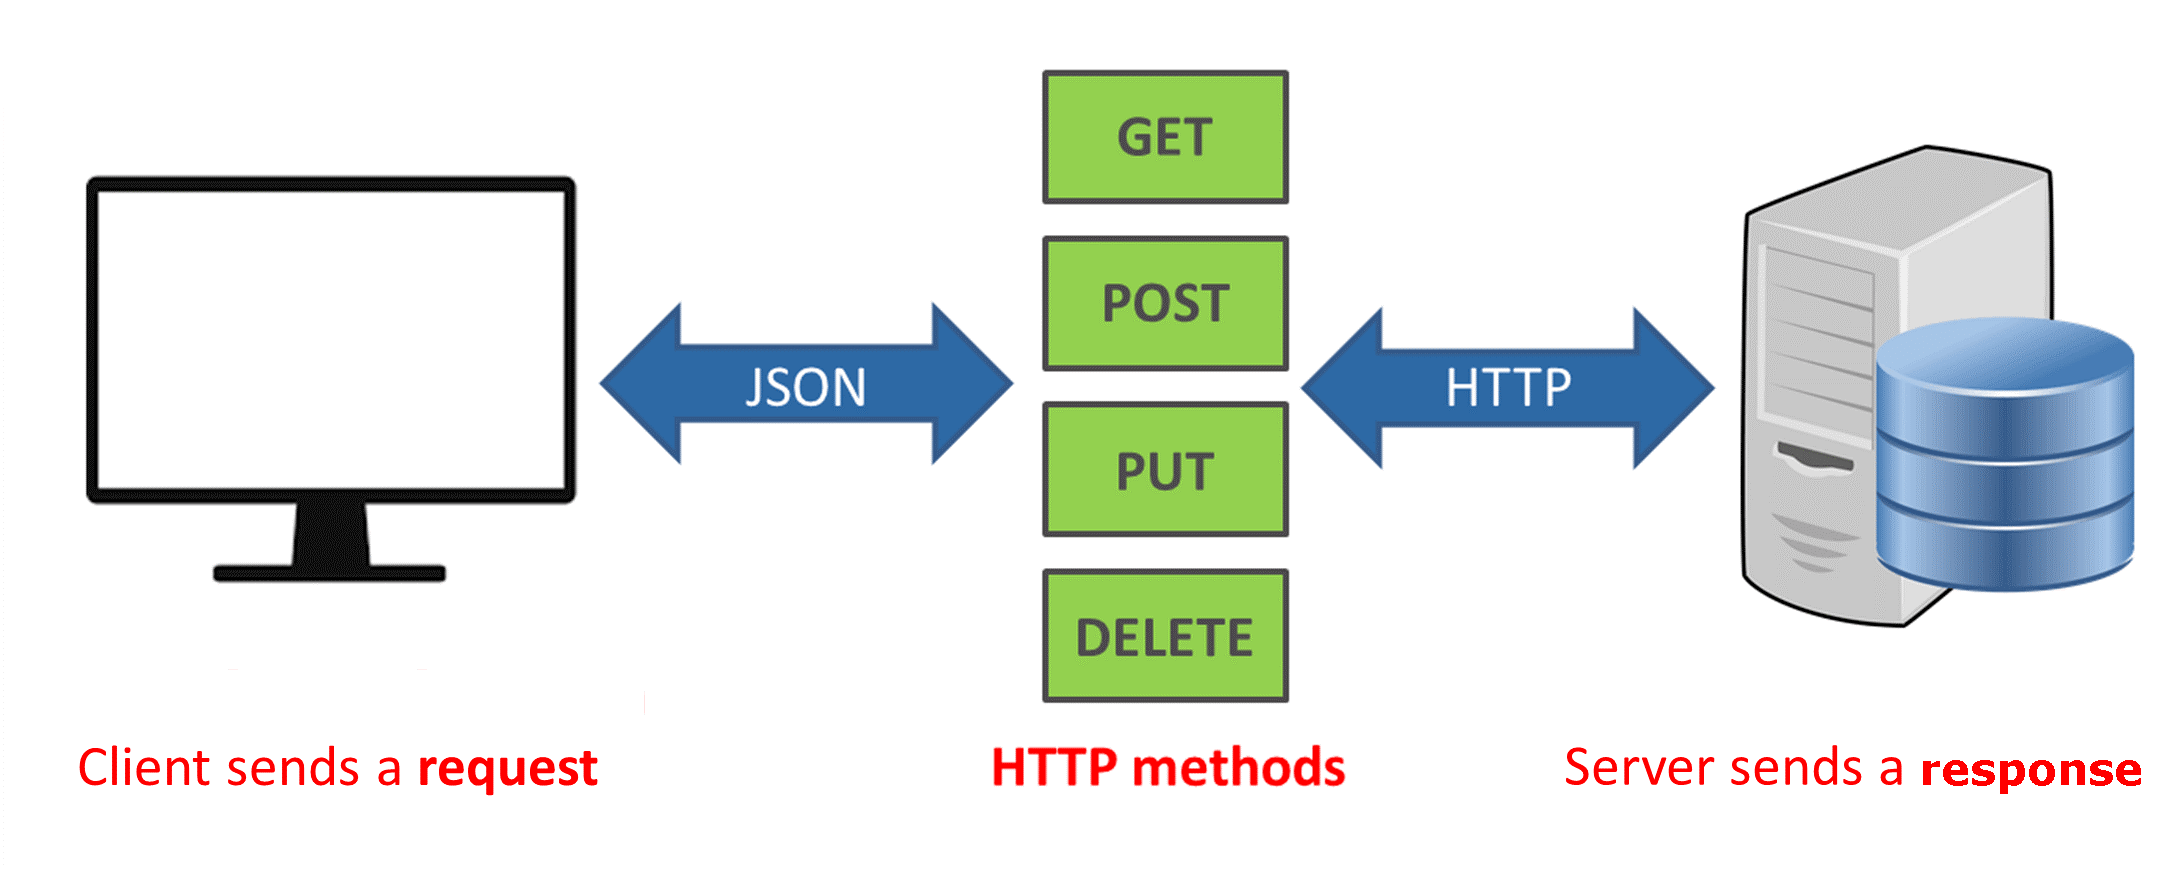
\includegraphics[width=0.9\textwidth]{./pics/restArchitecture.png}\\
\end{center}
\end{frame}

\section{Mangler og videreudvikling}

\begin{frame}
\frametitle{Mangler}
\begin{enumerate}
\item Frontend
\item design
\item Initiativrækkefølge
\end{enumerate}
\end{frame}

\begin{frame}
\frametitle{videreudvikling}
\begin{enumerate}
\item Condition-tracker
\item DragSelect
\item Drag \& drop
\item Flere Canvas lag
\item Få den op på en server
\item Markering fra lavere lag
\item Optimering
\item Sessioner
\item Sikkerhed
\item Tegne på canvas
\end{enumerate}
\end{frame}

\section{Reflektioner}

\begin{frame}
\frametitle{Refleksion}
Refleksioner
\end{frame}


\begin{frame}
\frametitle{Huskeliste til Svendeprøven}
\begin{itemize}
\item Vælg et mere begrænset Scope
\item forvent ikke mere end en prototype
\item Planlægning fritiden og sørg for at komme væk fra projektet.
\item Udvikl om dagen; dokumentér om eftermiddagen.
\end{itemize}
\end{frame}

\begin{frame}
\frametitle{Svendeprøve}
Svendeprøve
\end{frame}

\end{comment}

\begin{frame}
\frametitle{Spørgsmål}
Spørgsmål
\end{frame}

%%%%%%
%	Afslutning
%%%%%%

\end{document}